\chapter{Evaluation}
In this chapter, we aim to evaluate the expressiveness of Verlixir's design. First, we perform a qualatitive analysis of modeling classical distributed algorithms such as basic paxos in section \ref{sec:paxos} and the alternating-bit protocol in section \ref{sec:ab}. Section \ref{sec:vs} will delve into a comparison against current state-of-the-art model checking techniques for modern-day programming languages. Finally, we will explore the performance of Verlixir in a growing sytem in section \ref{sec:perf}.
\section{Analysing Distributed Systems}
Verifying the correctness of real-world distributed systems is a major motivation for this project. Critical real-time systems (such as in air-traffic control or healthcare  \cite{airlines,healthcare}) should not fail and should rely on rigerous verification techniques to guarantee production code is correct.  
\subsection{Basic Paxos} \label{sec:paxos}
Paxos is an example of a distributed algorithm \cite{paxos_simple}. It is a consensus algorithm, where many processes are tasked to agree on a value. Processes may propose what this value should be, but only one value should be agreed upon. The safety requirements (SR)s for consensus are:
\begin{itemize}
    \item \textbf{SR1}: Only a value that has been proposed may be chosen.
    \item \textbf{SR2}: Only a single value is chosen.
    \item \textbf{SR3}: A process never learns that a value has been chosen unless it actually has.
\end{itemize}
The system's liveness requirement is that a proposed value is eventually chosen and if a value if chosen then a process can learn the chosen value.
\subsubsection{Informal Specification}
There are many flavors to the paxos algorithm. We will informally present a basic, one-shot paxos. We introduce three roles in the system: proposer, acceptor and learner. The paxos algorithm performs two steps: prepare and accept. A proposer will broadcast a prepare message to all the acceptors, who will respond with a promise. When the proposer has received a promise from a quorum $q$ of acceptors, it will broadcast an accept message. If more than q acceptors accept, then the value is chosen, and the learners are informed.
\par
To evaluate the expressiveness of Verlixir, we first must write the paxos specification in LTLixir. The specifications of proposer, acceptor and learner are similar to those presented in pseudocode by Marzullo, Mei and Meling \cite{paxos_pseudocode}. We now present the key differences in our Elixir specification to a traditional paxos design.
%  For the remainder of the specification, we use the notations $A, \alpha, P, \pi, L, \lambda$ to respectively represent either a set or individual acceptor, proposer or learner.
\par
All processes contain two functions, a start function to introduce relevant initial configuration and a main loop to process messages. Every acceptor initializes an accepted proposal, value and minimum proposal to $-1$ and then processes $prepare$ and $accept$ messages until receiving a $terminate$ message, signifying consensus has been reached. A termination clause is important to ensure the completion of a round of paxos. A proposer receives its configuration in the form of a $bind$ message, before executing its protocol. If during phase two, when asking acceptors to accept a value, a quorum of acceptors rejects the proposal, the proposer will inform the system it has reached consensus on value $0$. Traditionally, the proposer would retry with a higher proposal number, but we aim to avoid infinite paths so instead introduce this terminating condition. The learner awaits a $learn$ message from all proposers. We only ever consider a single learner and the learner is also responsible for spawning the proposers and acceptors, choosing their values and assigning proposal numbers for the single round of paxos. We finally setup the learner such that it spawns three acceptors and two proposers. The learner decides the values the proposers will propose, which for this example will be $31$ and $42$. Of course, in a different context, these values may come from other sources within a larger system, however, notional values are sufficient for our purposes.
\par
With our implementation complete, we introduce the three safety requirements established. To achieve this, we introduce a value $final\_value$ which the learner receives from proposers. This value is initialized to $0$ and set to the agreed value of consensus. Let's specify the temporal formula required to express our safety requirements. We first introduce four predicates into our specification (note the use of $0$ both represents a state where consensus is unreached, or a value received from a rejected proposer).
\[
\begin{array}{l}
\text{predicate p: final\_value} == 31 \\
\text{predicate q: final\_value} == 42 \\
\text{predicate r: final\_value} \neq 0 \\
\text{predicate s: final\_value} == 0 \ \lor \ \text{final\_value} == 31 \ \lor \ \text{final\_value} == 42 \\
\end{array}
\]
We can now use the predicates to simplify the formulation of the safety requirements.
\begin{itemize}
    \item \textbf{SR1}: $\lozenge r$
    \item \textbf{SR2}: $\square ( ( p \rightarrow \neg \lozenge q ) \land ( q \rightarrow \neg \lozenge p ) )$ 
    \item \textbf{SR3}: $\square s$
\end{itemize}
We now have a complete specification of the basic paxos algorithm in LTLixir. Note that SR1 could be considered a liveness requirement, this is a result of slight modifications on the original SRs to align with our specific implementation decisions. We can run Verlixir on the model to verify the safety requirements. When we run the verification mode, we see that no SRs are violated. This justifies that both the informal paxos specification we defined is correct regarding our SRs and that the implementation of the specification is also correct.
\begin{lstlisting}[language=bash, xleftmargin=.3\linewidth]
    Model ran successfully. 0 error(s) found.
    The verifier terminated with no errors.
\end{lstlisting}
This gives a good indication that the expressiveness of Verlixir is sufficient to model and verify distributed systems. However, we also should investigate how Verlixir can express errors for a more complex system such as paxos. 
\subsubsection{Counter-example one}
We introduce a bug into the proposer's protocol. The proposer will now wait for a majority of acceptors to accept the proposal and only be rejected if a majority of acceptors reject the proposal. This is a violation of the protocol, as we only need a single rejection (within the accepting quorum) for a proposer to retry with a higher proposal number. We can now run the verifier on the model again to see if the bug is detected. Verlixir reports a violation of SR2, which is expected. In particular, we are told there is a violation SR2 due to $( final\_value == 31 )$. We can infer that the learner was informed the chosen value is $42$, but a later proposer informed the learner the chosen value is $31$. Verlixir detects this bug, informing us that SR2 was violated and then produces its counterexample. Digesting this counterexample can take some time, as the interleaving of process communication that triggers this bug involves approximately 50 messages and 800 steps. The full message log is available in the appendix. We will provide a simpler interpretation to help reason that Verlixir has correctly identified the bug (derived from the message log).
\begin{figure}[h]
    \centering
    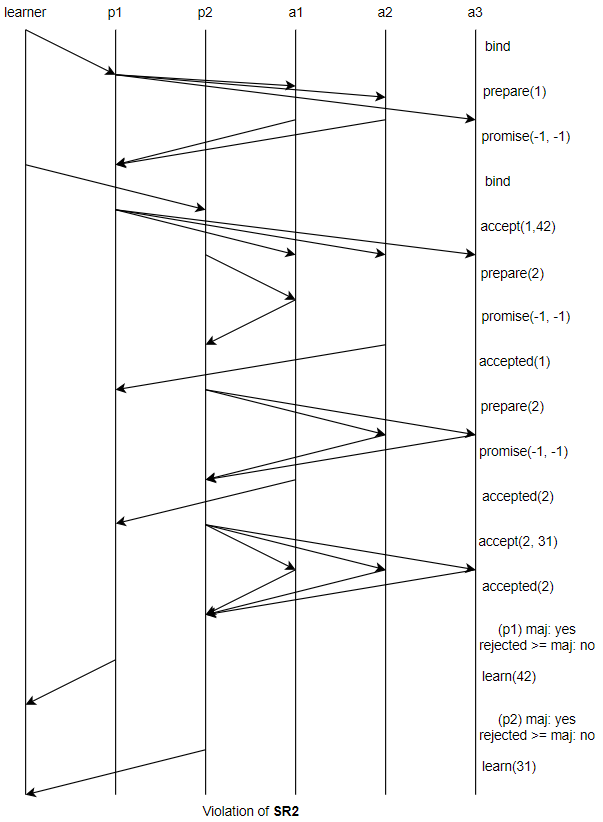
\includegraphics[width=0.7\textwidth]{images/paxos_1.png}
    \caption{Violation of paxos specification due to proposer bug. Note the figure only shows the ordering of receive events.}
    \label{fig:paxos_1}
\end{figure}
\subsubsection{Counter-example two}
We now explore a second counter-example, again, the paxos specification and message log can be found in the appendix. This time, we introduce a bug into the proposer, such that if the proposer receives a $\{prepared, proposalNumber, value\}$ message from an acceptor with a higher proposal number, it propagates this proposal number forward. A correct paxos implementation should keep the same proposal number, but propagate the value forward. We again get a violation of SR2, where the mutual exclusion of values is violated. The violation is the same as counter-example one but caused by a different interleaving. 
\par
TODO INSERT DIAGRAM OF MESSAGE INTERLEVING AND WHY IT FAILED?
\par
\subsection{Alternating-bit Protocol} \label{sec:ab}
\subsubsection{Informal Specification}
\subsubsection{Experimental Analysis}
\section{Verlixir vs state-of-the-art} \label{sec:vs}

\section{Performance} \label{sec:perf}